\subsection{Моделиране}

\subsubsection{Моделиране на тяга от витло и мотор}

За моделиране на моторът и витлото е приет опростеният модел:
Който моделира системата, коефициент на усливане и нискочестотен филтър.

\begin{figure}[htpb!]
    \centering
    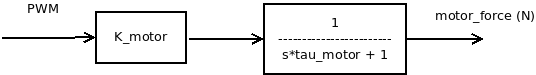
\includegraphics[width=0.7\textwidth]{motor_model}
    \caption{Опростен модел на витло и мотор}
    \label{fig:motor_model}
\end{figure}

\begin{equation}
    G_{motor}(s) = \frac{k_{motor}}{s \tau_{motor} + 1}
    \label{eqn:motor_model}
\end{equation}

Реално този модел не е добра апроксимация на тягата на моторите,
защото реалната характеристика е нелинейна и се променя спрямо множество параметри (напрежение на батерията, температура, налягане, вляжност, скорост),
но за неголеми времеви интервали и неголеми промени в входният сигнал статичната характеристика
може да бъде описана достатъчно добре, чрез линейната апроксимация (\autoref{eqn:motor_model}).


\subsubsection{Моделиране на платформа за управление на ъгъл на завъртане}

За моделиране на платформата за управление на ъгъл на завъртане (\autoref{fig:balance_force_diagram})
нека приемем, че въртящата час е пренебрежимо тънка, с дължина \(l\), и има маса \(M\). 
Ъгълът, който въртящата част сключва с хоризонта е означен с \(\phi\).
Във края на рамената се намират безчетковите мотори и витлата, моделирани, като концентрирани
маси с големина \(m\), като всеки от тях има сила на тягата означена с \(F_1, F_2\) респективно.
Триенето с въртящата ос е моделирано с коефициентът на триене \(C\).

\begin{figure}[htpb!]
    \centering
    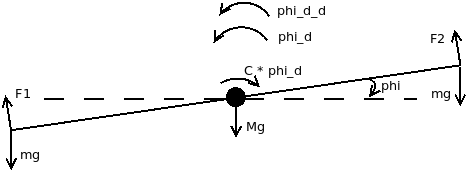
\includegraphics[width=0.7\textwidth]{balance_force_diagram}
    \caption{Диаграма на платформа за управление на ъгъл на завъртане}
    \label{fig:balance_force_diagram}
\end{figure}

От втори закон на Нютон \autoref{eqn:newton1}, 
\begin{equation}
    I \ddot{\phi} = \sum_i \tau_i
    \label{eqn:newton1}
\end{equation}
От където следва:
\begin{equation}
    I \ddot{\phi} = F_2*\frac{l}{2} - F_1*\frac{l}{2} - C \dot{\phi}
    \label{eqn:newton1_expand}
\end{equation}
Нека:
\begin{equation}
    F_2 = F_0 + \delta f, F_1 = F_0 - \delta f 
\end{equation}
След като заместим в \autoref{eqn:newton1_expand}
\begin{equation}
    I \ddot{\phi} = (F_0 + \delta f)*\frac{l}{2} - (F_0 - \delta f)*\frac{l}{2} - C \dot{\phi}
\end{equation}
Плучаваме:
\begin{equation}
    I \ddot{\phi} + C \dot{\phi} = l * \delta f
\end{equation}
Което опростява системата до линейна SISO система.

Апроксимираме инерционният момент \(I\) като :
\begin{align}
    I &= I_{rod} + 2*I_{motor}\\
    I &= \frac{1}{12}Ml^2 + 2m(\frac{l}{2})^2 \\
    I &= \frac{l^2}{12}(M + 6m)
\end{align}

При нулеви начални условия след трансформация на Лаплас получаваме:
\begin{equation}
    s^2 I \bar{\Phi}(s) + s C \bar{\Phi}(s) = l * \bar{\delta f}(s) 
\end{equation}
От където получаваме предавателната функция:
\begin{equation}
    G_{platform}(s) = \frac{\bar{\Phi}(s)}{\bar{\delta f }(s)} = \frac{l}{s ( s I + C)}
\end{equation}

За получаване на предавателната функция на отворената система:
\begin{equation}
    G_{sys} = G_{motor}(s)G_{platform}(s) = 
    \frac{k_{motor} l}{s( s I + C)(s \tau_{motor} + 1)} 
\end{equation}

\subsection{Компенсация на сензорни отмествания}

\subsubsection{Компенсация на жироскопен дрейф}
\FloatBarrier
Жироскопите обикновено не са силно зашумени за разлика от
акселерометрите, но имат своите недсостатъци.
Основен проблем при жироскопите е т.нар. жироскопен дрейф.
В неподвижно състояние жироскопът показва малко постоянно завъртане в някоя посока.
Жироскопният дрейф зависи основно от температурата.

За да калибрираме и занулим стойностите на жироскопа
се налага да направим полиномиална компенсация по температура.

За целта жироскопа е ухладен до \(0^{\circ}C\)
след което е поставен неподвижно бавно да се загрее в продължение на 45мин до стайна температура.
През цялото време събираме данните от жироскопа и измерената от бордовия термометър температура.
След приключване на експеримента използваме матлаб за намиране на полином,
който точно описва получените данни за всяка от осите.

\begin{figure}[htpb!]
    \centering
    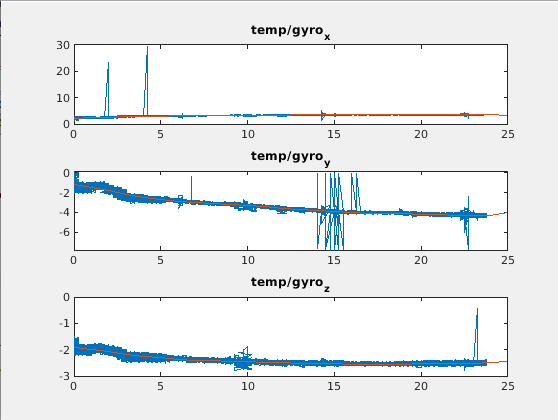
\includegraphics[width=0.9\textwidth]{gyro_drift_calibrate}
    \caption{Жироскопен дрейф спрямо температура и полиномиална компенсация спрямо температура}
    \label{fig:gyro_drift_calibrate}
\end{figure}

\begin{lstlisting}[language=matlab, caption={Получени полиноми за коменсация на жироскопният дрейф}, label={lst:gyro_drift_poly}]

    p_x =

     -42.6978e-9  3.7797e-6  -131.8066e-006  2.2717e-3  -19.5918e-3  67.9744e-3  95.1384e-3  2.2440e+0

  p_y =
  
      87.1716e-9  -7.6384e-6  263.1019e-006  -4.4660e-3  37.8030e-3  -129.2365e-3  -191.6577e-3  -1.1695e+0
  p_z =
  
      15.9591e-9  -1.4613e-6  53.0721e-006  -961.5439e-6  8.8365e-3  -33.3197e-3  -44.0584e-003  -1.9076e+0

\end{lstlisting}


\FloatBarrier


\subsubsection{Компенсация на магнитни отмествания от околната среда}
\FloatBarrier
Магнитометрите имат постоянно отместване поради средата в която се намират.
Това отместване се дължи на металните и магнитни обекти,
както и всички електромагнитни смущения причинени от заобикалящата ни среда.
Поради факта, че в близката ни околна среда тези смущения са постоянни, което означава, че ние можем да ги компенсираме статично.


За целта поставяме сензора в нормална позиция и бавно го завъртаме, като се стараем да покрием възможно най-много ъглови комбинации.
След получаване на данните виждаме, че те образуват Елипсоид с отместен център.
Използваме техника на Мерайо.
Идентифицираме елипсоида и отместването на центъра,
след което правим трансформация елипсоид-сфера,
след което изваждаме отместването на центъра.
Верифицираме резултатът, като виждаме, че всички измерени точки са в допостим диапазон от повърхността на сфера с център 0 и радиус 1.

\begin{figure}[htpb!]
    \centering
    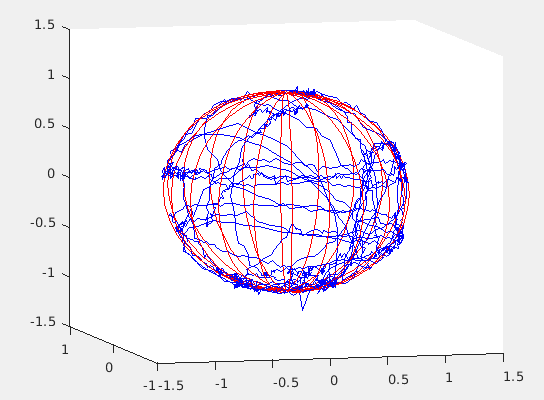
\includegraphics[width=0.9\textwidth]{mag_calibration}
    \caption{Компенсирани данни получени от магнитометър}
    \label{fig:mag_calibration}
\end{figure}

\begin{lstlisting}[language=matlab, caption={Получени трансформация елипсоид-сфера и отместване на център}, label={lst:mag_cal_trans}]

    U =

    21.4229e+000   837.9000e-003     3.0861e+000
     0.0000e+000    21.6201e+000     2.0207e+000
     0.0000e+000     0.0000e+000    27.2441e+000

    c =

    -1.6000e-003
    19.9000e-003
    45.7000e-003

\end{lstlisting}



\FloatBarrier


